% Options for packages loaded elsewhere
% Options for packages loaded elsewhere
\PassOptionsToPackage{unicode}{hyperref}
\PassOptionsToPackage{hyphens}{url}
\PassOptionsToPackage{dvipsnames,svgnames,x11names}{xcolor}
%
\documentclass[
  letterpaper,
  DIV=11,
  numbers=noendperiod]{scrartcl}
\usepackage{xcolor}
\usepackage{amsmath,amssymb}
\setcounter{secnumdepth}{-\maxdimen} % remove section numbering
\usepackage{iftex}
\ifPDFTeX
  \usepackage[T1]{fontenc}
  \usepackage[utf8]{inputenc}
  \usepackage{textcomp} % provide euro and other symbols
\else % if luatex or xetex
  \usepackage{unicode-math} % this also loads fontspec
  \defaultfontfeatures{Scale=MatchLowercase}
  \defaultfontfeatures[\rmfamily]{Ligatures=TeX,Scale=1}
\fi
\usepackage{lmodern}
\ifPDFTeX\else
  % xetex/luatex font selection
\fi
% Use upquote if available, for straight quotes in verbatim environments
\IfFileExists{upquote.sty}{\usepackage{upquote}}{}
\IfFileExists{microtype.sty}{% use microtype if available
  \usepackage[]{microtype}
  \UseMicrotypeSet[protrusion]{basicmath} % disable protrusion for tt fonts
}{}
\makeatletter
\@ifundefined{KOMAClassName}{% if non-KOMA class
  \IfFileExists{parskip.sty}{%
    \usepackage{parskip}
  }{% else
    \setlength{\parindent}{0pt}
    \setlength{\parskip}{6pt plus 2pt minus 1pt}}
}{% if KOMA class
  \KOMAoptions{parskip=half}}
\makeatother
% Make \paragraph and \subparagraph free-standing
\makeatletter
\ifx\paragraph\undefined\else
  \let\oldparagraph\paragraph
  \renewcommand{\paragraph}{
    \@ifstar
      \xxxParagraphStar
      \xxxParagraphNoStar
  }
  \newcommand{\xxxParagraphStar}[1]{\oldparagraph*{#1}\mbox{}}
  \newcommand{\xxxParagraphNoStar}[1]{\oldparagraph{#1}\mbox{}}
\fi
\ifx\subparagraph\undefined\else
  \let\oldsubparagraph\subparagraph
  \renewcommand{\subparagraph}{
    \@ifstar
      \xxxSubParagraphStar
      \xxxSubParagraphNoStar
  }
  \newcommand{\xxxSubParagraphStar}[1]{\oldsubparagraph*{#1}\mbox{}}
  \newcommand{\xxxSubParagraphNoStar}[1]{\oldsubparagraph{#1}\mbox{}}
\fi
\makeatother

\usepackage{color}
\usepackage{fancyvrb}
\newcommand{\VerbBar}{|}
\newcommand{\VERB}{\Verb[commandchars=\\\{\}]}
\DefineVerbatimEnvironment{Highlighting}{Verbatim}{commandchars=\\\{\}}
% Add ',fontsize=\small' for more characters per line
\usepackage{framed}
\definecolor{shadecolor}{RGB}{241,243,245}
\newenvironment{Shaded}{\begin{snugshade}}{\end{snugshade}}
\newcommand{\AlertTok}[1]{\textcolor[rgb]{0.68,0.00,0.00}{#1}}
\newcommand{\AnnotationTok}[1]{\textcolor[rgb]{0.37,0.37,0.37}{#1}}
\newcommand{\AttributeTok}[1]{\textcolor[rgb]{0.40,0.45,0.13}{#1}}
\newcommand{\BaseNTok}[1]{\textcolor[rgb]{0.68,0.00,0.00}{#1}}
\newcommand{\BuiltInTok}[1]{\textcolor[rgb]{0.00,0.23,0.31}{#1}}
\newcommand{\CharTok}[1]{\textcolor[rgb]{0.13,0.47,0.30}{#1}}
\newcommand{\CommentTok}[1]{\textcolor[rgb]{0.37,0.37,0.37}{#1}}
\newcommand{\CommentVarTok}[1]{\textcolor[rgb]{0.37,0.37,0.37}{\textit{#1}}}
\newcommand{\ConstantTok}[1]{\textcolor[rgb]{0.56,0.35,0.01}{#1}}
\newcommand{\ControlFlowTok}[1]{\textcolor[rgb]{0.00,0.23,0.31}{\textbf{#1}}}
\newcommand{\DataTypeTok}[1]{\textcolor[rgb]{0.68,0.00,0.00}{#1}}
\newcommand{\DecValTok}[1]{\textcolor[rgb]{0.68,0.00,0.00}{#1}}
\newcommand{\DocumentationTok}[1]{\textcolor[rgb]{0.37,0.37,0.37}{\textit{#1}}}
\newcommand{\ErrorTok}[1]{\textcolor[rgb]{0.68,0.00,0.00}{#1}}
\newcommand{\ExtensionTok}[1]{\textcolor[rgb]{0.00,0.23,0.31}{#1}}
\newcommand{\FloatTok}[1]{\textcolor[rgb]{0.68,0.00,0.00}{#1}}
\newcommand{\FunctionTok}[1]{\textcolor[rgb]{0.28,0.35,0.67}{#1}}
\newcommand{\ImportTok}[1]{\textcolor[rgb]{0.00,0.46,0.62}{#1}}
\newcommand{\InformationTok}[1]{\textcolor[rgb]{0.37,0.37,0.37}{#1}}
\newcommand{\KeywordTok}[1]{\textcolor[rgb]{0.00,0.23,0.31}{\textbf{#1}}}
\newcommand{\NormalTok}[1]{\textcolor[rgb]{0.00,0.23,0.31}{#1}}
\newcommand{\OperatorTok}[1]{\textcolor[rgb]{0.37,0.37,0.37}{#1}}
\newcommand{\OtherTok}[1]{\textcolor[rgb]{0.00,0.23,0.31}{#1}}
\newcommand{\PreprocessorTok}[1]{\textcolor[rgb]{0.68,0.00,0.00}{#1}}
\newcommand{\RegionMarkerTok}[1]{\textcolor[rgb]{0.00,0.23,0.31}{#1}}
\newcommand{\SpecialCharTok}[1]{\textcolor[rgb]{0.37,0.37,0.37}{#1}}
\newcommand{\SpecialStringTok}[1]{\textcolor[rgb]{0.13,0.47,0.30}{#1}}
\newcommand{\StringTok}[1]{\textcolor[rgb]{0.13,0.47,0.30}{#1}}
\newcommand{\VariableTok}[1]{\textcolor[rgb]{0.07,0.07,0.07}{#1}}
\newcommand{\VerbatimStringTok}[1]{\textcolor[rgb]{0.13,0.47,0.30}{#1}}
\newcommand{\WarningTok}[1]{\textcolor[rgb]{0.37,0.37,0.37}{\textit{#1}}}

\usepackage{longtable,booktabs,array}
\usepackage{calc} % for calculating minipage widths
% Correct order of tables after \paragraph or \subparagraph
\usepackage{etoolbox}
\makeatletter
\patchcmd\longtable{\par}{\if@noskipsec\mbox{}\fi\par}{}{}
\makeatother
% Allow footnotes in longtable head/foot
\IfFileExists{footnotehyper.sty}{\usepackage{footnotehyper}}{\usepackage{footnote}}
\makesavenoteenv{longtable}
\usepackage{graphicx}
\makeatletter
\newsavebox\pandoc@box
\newcommand*\pandocbounded[1]{% scales image to fit in text height/width
  \sbox\pandoc@box{#1}%
  \Gscale@div\@tempa{\textheight}{\dimexpr\ht\pandoc@box+\dp\pandoc@box\relax}%
  \Gscale@div\@tempb{\linewidth}{\wd\pandoc@box}%
  \ifdim\@tempb\p@<\@tempa\p@\let\@tempa\@tempb\fi% select the smaller of both
  \ifdim\@tempa\p@<\p@\scalebox{\@tempa}{\usebox\pandoc@box}%
  \else\usebox{\pandoc@box}%
  \fi%
}
% Set default figure placement to htbp
\def\fps@figure{htbp}
\makeatother





\setlength{\emergencystretch}{3em} % prevent overfull lines

\providecommand{\tightlist}{%
  \setlength{\itemsep}{0pt}\setlength{\parskip}{0pt}}



 


\KOMAoption{captions}{tableheading}
\makeatletter
\@ifpackageloaded{caption}{}{\usepackage{caption}}
\AtBeginDocument{%
\ifdefined\contentsname
  \renewcommand*\contentsname{Table of contents}
\else
  \newcommand\contentsname{Table of contents}
\fi
\ifdefined\listfigurename
  \renewcommand*\listfigurename{List of Figures}
\else
  \newcommand\listfigurename{List of Figures}
\fi
\ifdefined\listtablename
  \renewcommand*\listtablename{List of Tables}
\else
  \newcommand\listtablename{List of Tables}
\fi
\ifdefined\figurename
  \renewcommand*\figurename{Figure}
\else
  \newcommand\figurename{Figure}
\fi
\ifdefined\tablename
  \renewcommand*\tablename{Table}
\else
  \newcommand\tablename{Table}
\fi
}
\@ifpackageloaded{float}{}{\usepackage{float}}
\floatstyle{ruled}
\@ifundefined{c@chapter}{\newfloat{codelisting}{h}{lop}}{\newfloat{codelisting}{h}{lop}[chapter]}
\floatname{codelisting}{Listing}
\newcommand*\listoflistings{\listof{codelisting}{List of Listings}}
\makeatother
\makeatletter
\makeatother
\makeatletter
\@ifpackageloaded{caption}{}{\usepackage{caption}}
\@ifpackageloaded{subcaption}{}{\usepackage{subcaption}}
\makeatother
\usepackage{bookmark}
\IfFileExists{xurl.sty}{\usepackage{xurl}}{} % add URL line breaks if available
\urlstyle{same}
\hypersetup{
  pdftitle={Informe Técnico Final: Plataforma de Micro-empleos Universitarios},
  pdfauthor={Equipo de Desarrollo},
  colorlinks=true,
  linkcolor={blue},
  filecolor={Maroon},
  citecolor={Blue},
  urlcolor={Blue},
  pdfcreator={LaTeX via pandoc}}


\title{Informe Técnico Final: Plataforma de Micro-empleos
Universitarios}
\author{Equipo de Desarrollo}
\date{}
\begin{document}
\maketitle


\section{Introducción}\label{introducciuxf3n}

El presente documento detalla la arquitectura, diseño e implementación
de la Plataforma de Micro-empleos Universitarios. Este sistema integra
soluciones móviles y web para facilitar la conexión entre empresas que
ofrecen trabajos cortos y estudiantes universitarios que buscan
oportunidades laborales flexibles.

La arquitectura del sistema se basa en un enfoque de microservicios para
garantizar la escalabilidad y la modularidad. Un componente crítico de
esta arquitectura es el servicio de validación de estudiantes, el cual
interactúa con una base de datos externa de la Universidad para
certificar que los postulantes son alumnos activos.

La seguridad es un pilar fundamental, implementando autenticación
mediante JSON Web Tokens (JWT) para el manejo de sesiones y un Token de
Verificación adicional que asegura la integridad del proceso de
postulación. La solución se compone de una aplicación móvil desarrollada
en React Native, un frontend web, y un backend robusto en Node.js.

\section{Arquitectura del Sistema (Modelo
C4)}\label{arquitectura-del-sistema-modelo-c4}

A continuación, se presentan los diagramas de arquitectura utilizando el
modelo C4 para visualizar los diferentes niveles de abstracción del
sistema.

\subsection{Nivel 2: Diagrama de
Contenedores}\label{nivel-2-diagrama-de-contenedores}

Este diagrama muestra los contenedores de software de alto nivel y cómo
interactúan entre sí y con los actores externos.

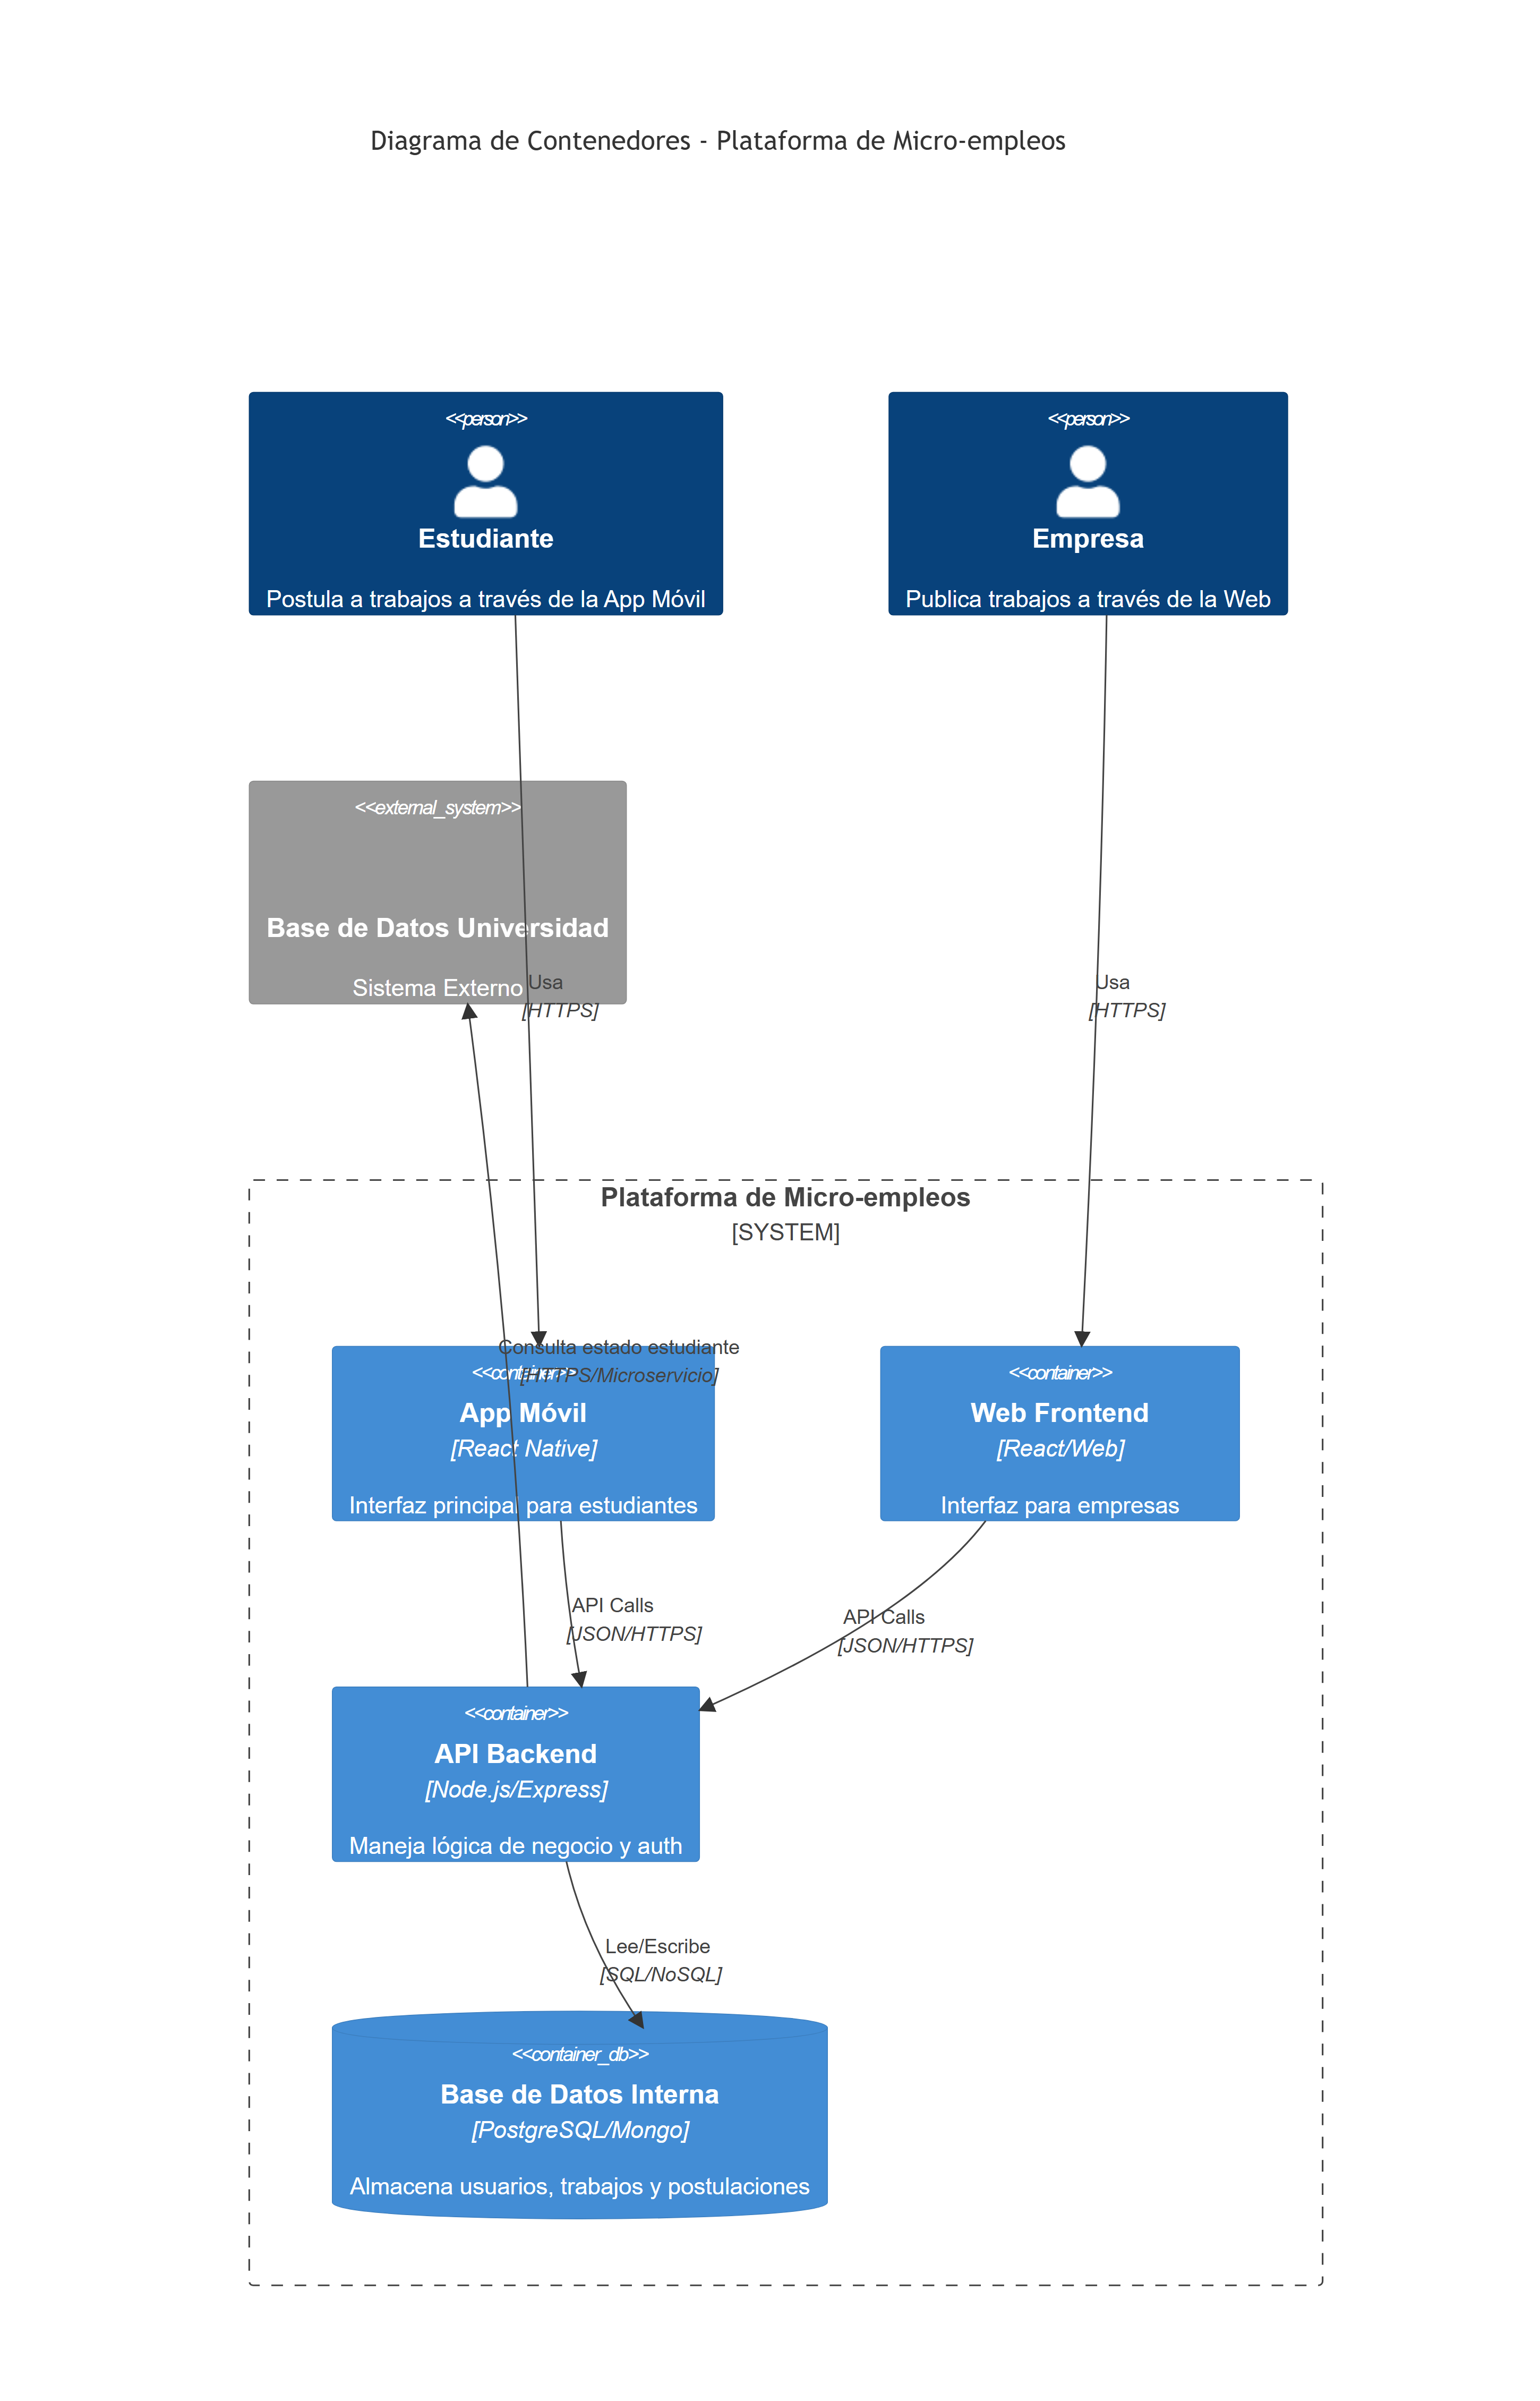
\includegraphics[width=9.85in,height=15.36in]{informe_final_files/figure-latex/mermaid-figure-1.png}

\subsection{Nivel 3: Diagrama de Componentes (App
Móvil)}\label{nivel-3-diagrama-de-componentes-app-muxf3vil}

Desglose de la aplicación móvil en sus componentes principales.

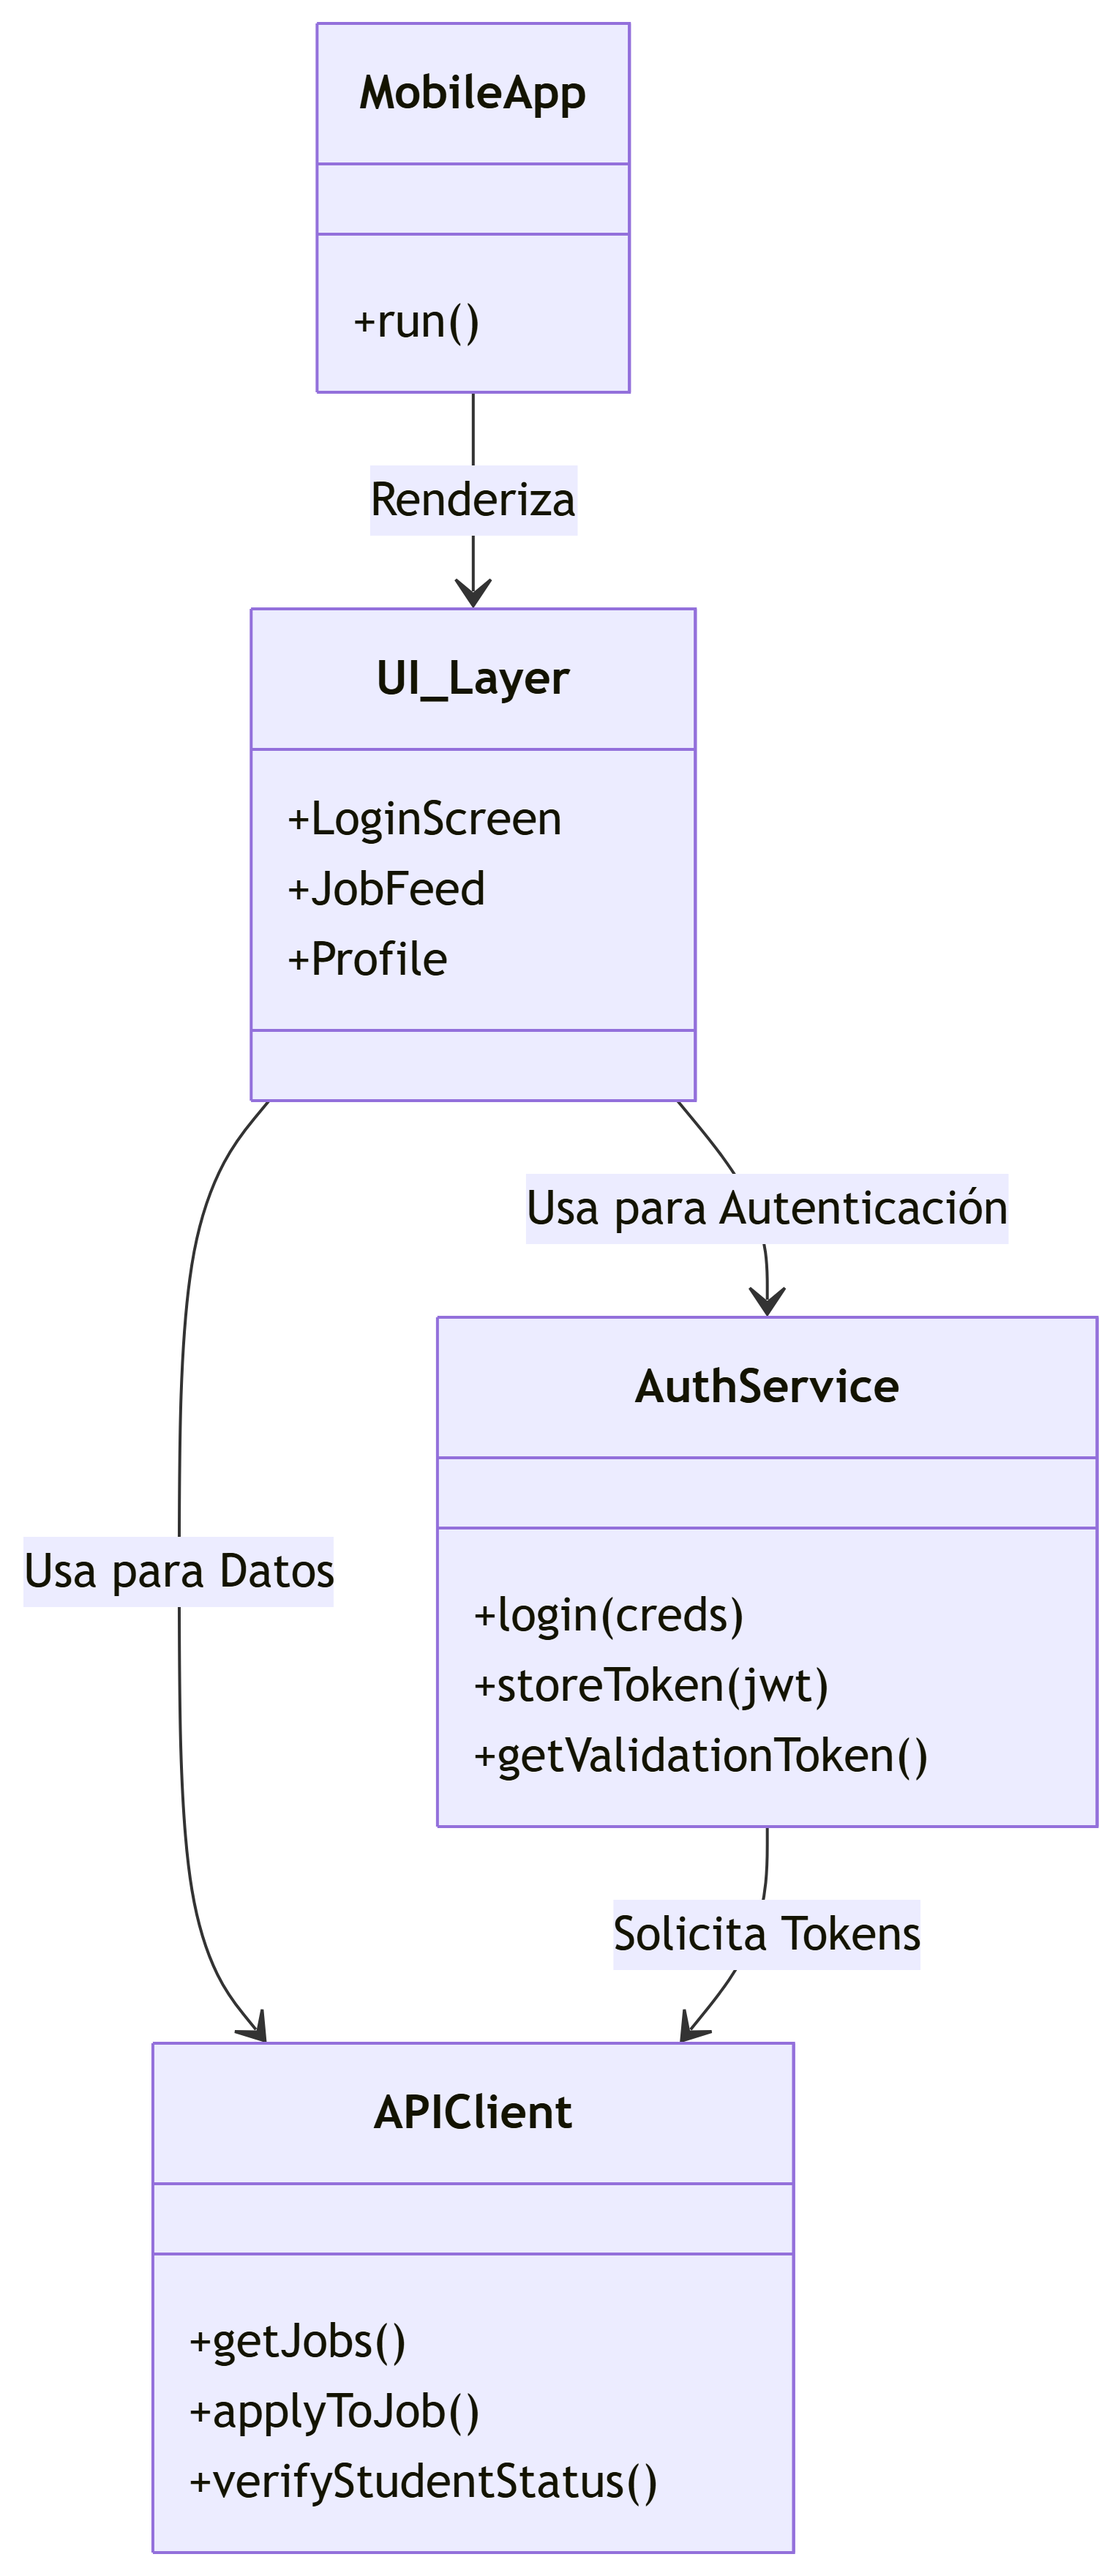
\includegraphics[width=3.99in,height=9.17in]{informe_final_files/figure-latex/mermaid-figure-3.png}

\subsection{Nivel 4: Diagrama de Código (Login y
Registro)}\label{nivel-4-diagrama-de-cuxf3digo-login-y-registro}

Detalle de las clases involucradas en el proceso de autenticación.

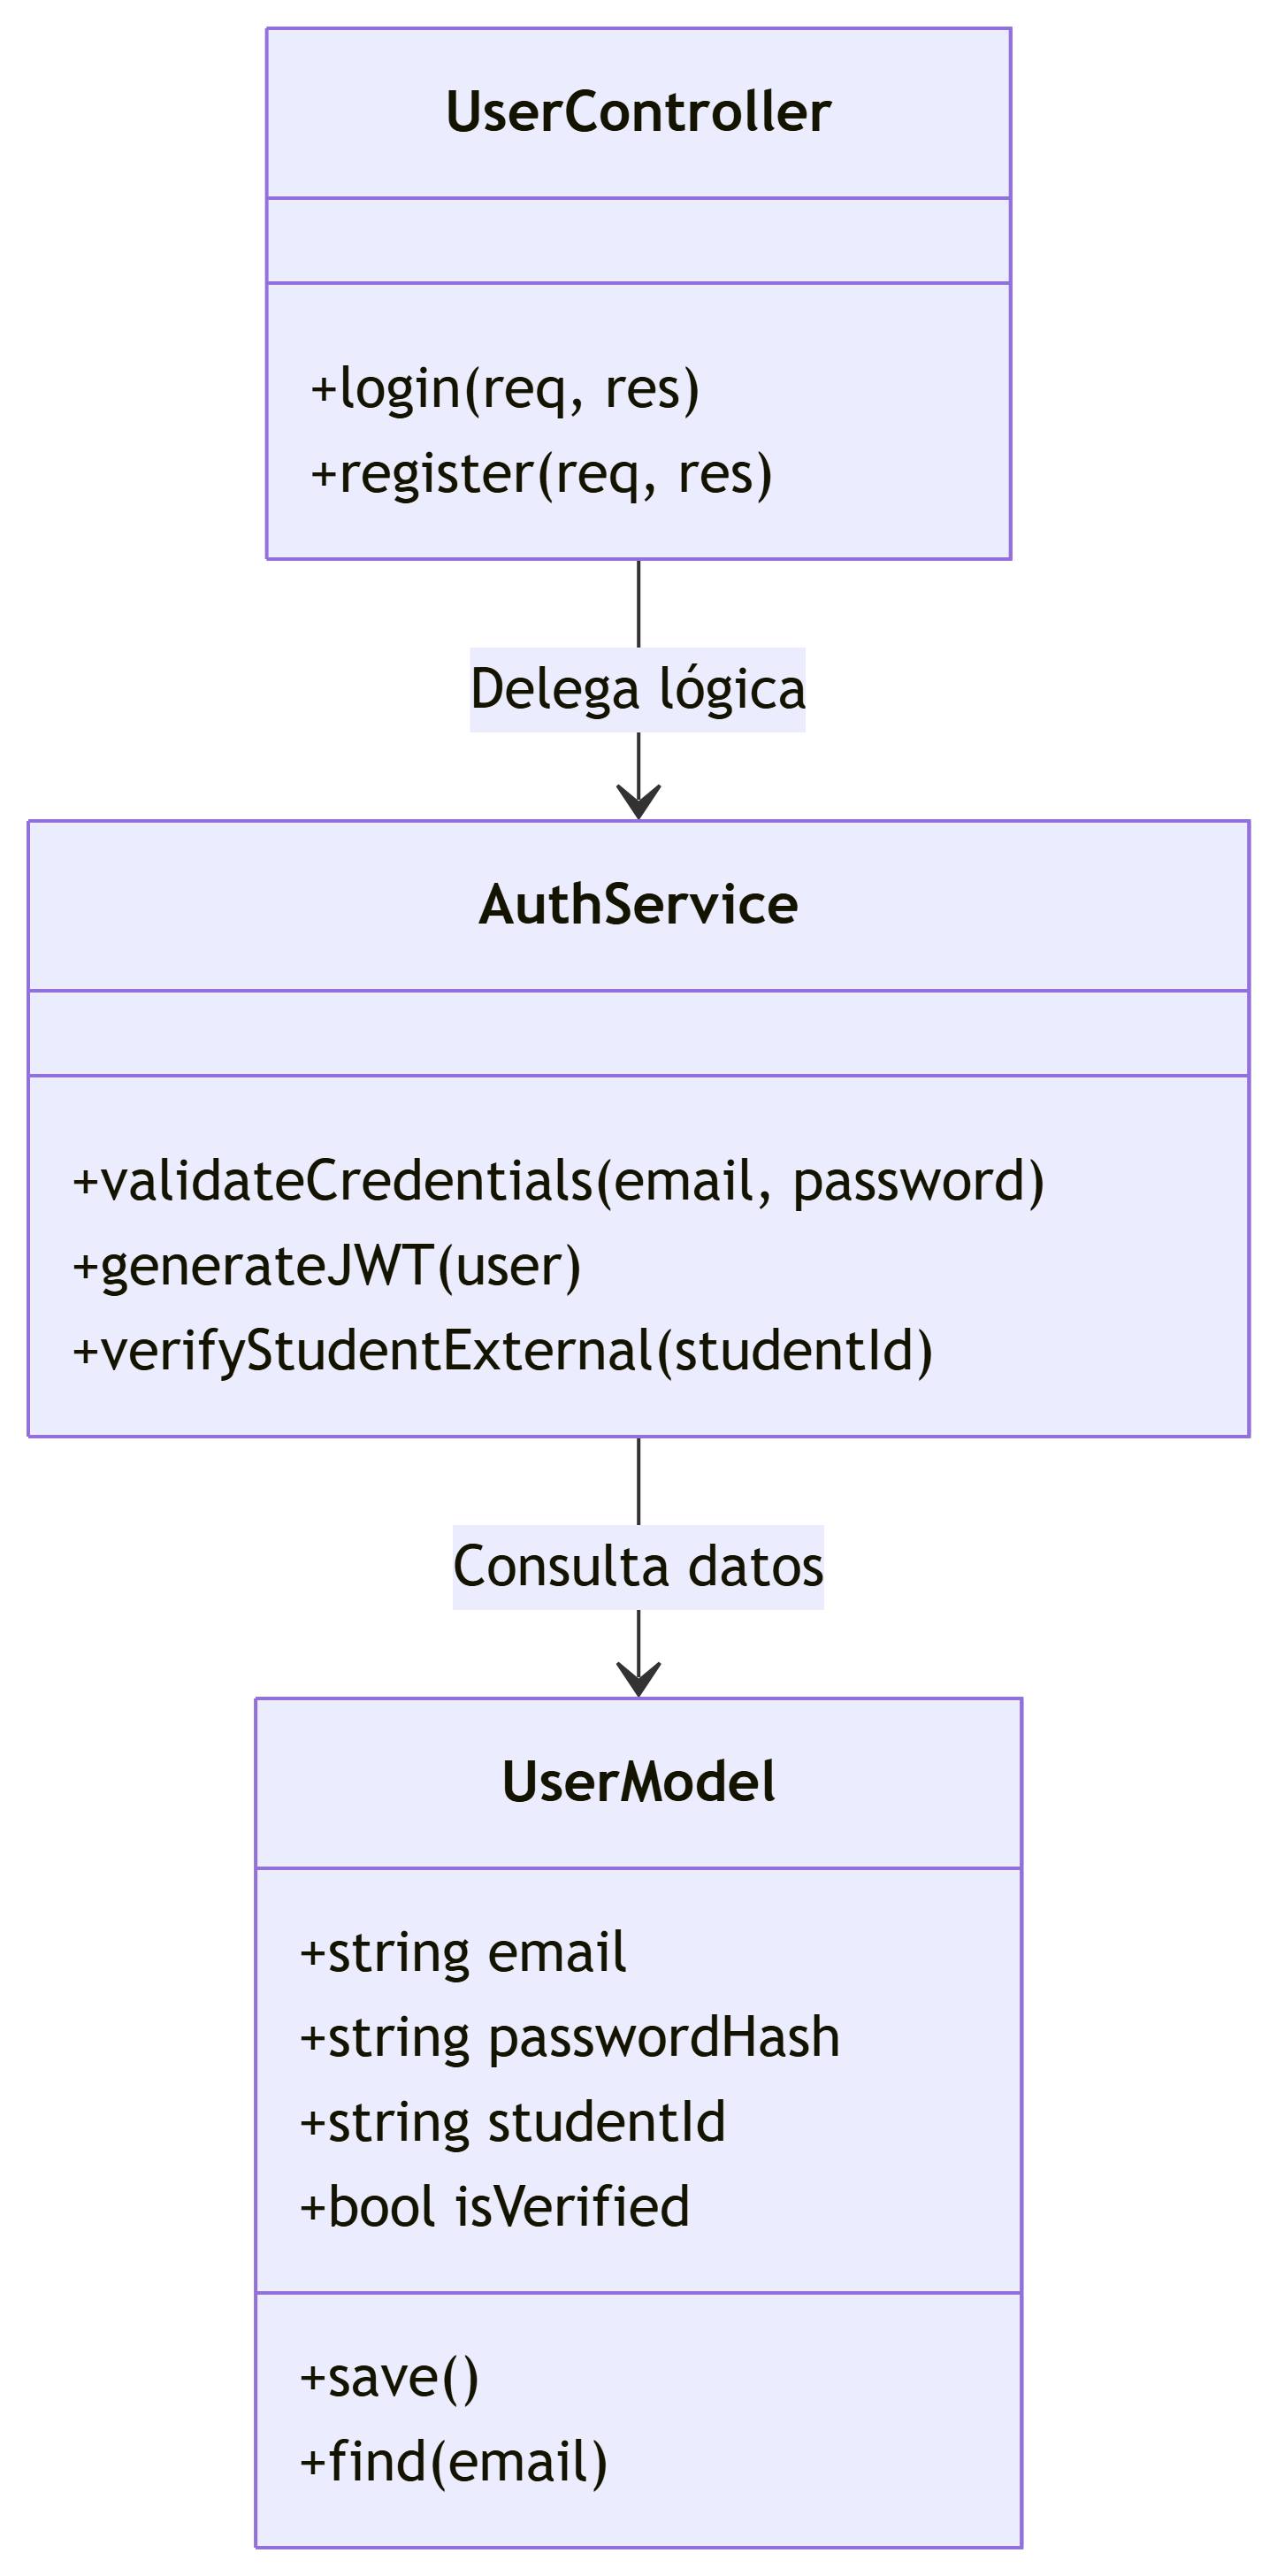
\includegraphics[width=3.76in,height=7.58in]{informe_final_files/figure-latex/mermaid-figure-2.png}

\section{Manual de Usuario y Guía de
Instalación}\label{manual-de-usuario-y-guuxeda-de-instalaciuxf3n}

\subsection{Configuración del Entorno
Móvil}\label{configuraciuxf3n-del-entorno-muxf3vil}

Para conectar la aplicación móvil con el backend, es necesario
configurar la dirección IP del servidor en el archivo de entorno.

\begin{enumerate}
\def\labelenumi{\arabic{enumi}.}
\tightlist
\item
  Navegue a la carpeta \texttt{/mobile}.
\item
  Cree o edite el archivo \texttt{.env}.
\item
  Defina la variable \texttt{API\_URL} con la IP de su máquina local o
  servidor de desarrollo.
\end{enumerate}

\begin{Shaded}
\begin{Highlighting}[]
\CommentTok{\# Ejemplo de contenido .env en /mobile}
\VariableTok{API\_URL}\OperatorTok{=}\NormalTok{http://192.168.1.50:3000/api}
\end{Highlighting}
\end{Shaded}

\subsection{Comandos de Instalación}\label{comandos-de-instalaciuxf3n}

Siga estos pasos para desplegar el entorno de desarrollo localmente.

\subsubsection{Backend}\label{backend}

\begin{Shaded}
\begin{Highlighting}[]
\BuiltInTok{cd}\NormalTok{ backend}
\ExtensionTok{npm}\NormalTok{ install}
\ExtensionTok{npm}\NormalTok{ run dev}
\CommentTok{\# El servidor iniciará en el puerto 3000 por defecto}
\end{Highlighting}
\end{Shaded}

\subsubsection{Mobile App (React Native)}\label{mobile-app-react-native}

Asegúrese de tener un emulador Android/iOS corriendo o un dispositivo
físico conectado.

\begin{Shaded}
\begin{Highlighting}[]
\BuiltInTok{cd}\NormalTok{ mobile}
\ExtensionTok{npm}\NormalTok{ install}
\ExtensionTok{npx}\NormalTok{ react{-}native run{-}android}
\CommentTok{\# O para iOS}
\CommentTok{\# npx react{-}native run{-}ios}
\end{Highlighting}
\end{Shaded}

\section{Pruebas de Integración}\label{pruebas-de-integraciuxf3n}

A continuación se detallan los casos de prueba para validar la
integración entre los servicios.

\begin{longtable}[]{@{}
  >{\centering\arraybackslash}p{(\linewidth - 8\tabcolsep) * \real{0.1636}}
  >{\raggedright\arraybackslash}p{(\linewidth - 8\tabcolsep) * \real{0.2000}}
  >{\raggedright\arraybackslash}p{(\linewidth - 8\tabcolsep) * \real{0.1273}}
  >{\raggedright\arraybackslash}p{(\linewidth - 8\tabcolsep) * \real{0.3636}}
  >{\raggedright\arraybackslash}p{(\linewidth - 8\tabcolsep) * \real{0.1455}}@{}}
\toprule\noalign{}
\begin{minipage}[b]{\linewidth}\centering
ID Caso
\end{minipage} & \begin{minipage}[b]{\linewidth}\raggedright
Escenario
\end{minipage} & \begin{minipage}[b]{\linewidth}\raggedright
Pasos
\end{minipage} & \begin{minipage}[b]{\linewidth}\raggedright
Resultado Esperado
\end{minipage} & \begin{minipage}[b]{\linewidth}\raggedright
Estado
\end{minipage} \\
\midrule\noalign{}
\endhead
\bottomrule\noalign{}
\endlastfoot
\textbf{TI-01} & \textbf{Validación de estudiante regular} & 1.
Estudiante ingresa credenciales.2. Sistema consulta DB Universidad.3. DB
Universidad confirma estado ``Activo''. & Se genera Token de
Verificación y se permite acceso completo. & ✅ Aprobado \\
\textbf{TI-02} & \textbf{Validación de estudiante inactivo} & 1.
Estudiante ingresa credenciales.2. Sistema consulta DB Universidad.3. DB
Universidad retorna estado ``Inactivo''. & Login permitido pero
postulación bloqueada. Mensaje de error visible. & ✅ Aprobado \\
\textbf{TI-03} & \textbf{Postulación exitosa desde móvil} & 1.
Estudiante selecciona oferta.2. Clic en ``Postular''.3. App envía JWT +
Token Verificación. & Backend registra postulación y notifica éxito. &
✅ Aprobado \\
\textbf{TI-04} & \textbf{Error de conexión con Backend} & 1. Abrir App
sin conexión a internet o backend caído.2. Intentar navegar. & App
muestra pantalla de ``Sin Conexión'' o ``Reintentar''. & ⚠️ Pendiente \\
\end{longtable}




\end{document}
